%====================================================================
%	CAPA, CREDITOS & PREFACIO
%====================================================================
%

%====================================================================
%	Informacoes sobre o evento
%====================================================================

\def\edverao{edicao_verao} %coloque aqui a edicao do verao
\def\edworkshop{edicao_workshop} %coloque aqui a edicao do workshop
\def\datainic{data_inicio_evento}  %coloque aqui a data de inicio do workshop
\def\datafim{data_fim_evento} %coloque aqui a data de termino do workshop
\def\ano{ano_realizacao_evento} %coloque aqui ano do verao 
%
%====================================================================
%	Informacoes sobre Gestores e Coordenadores
%====================================================================
\def\reitor{M\'{a}rcia Abrah\~{a}o Moura} %reitor da UnB
\def\dirIE{Gladston Luiz da Silva} %diretor do IE
\def\chefMAT{Ricardo Ruviaro} %chefe do MAT
\def\coordext{Regina da Silva Pina Neves} %coordenador de extensao
\def\coordpos{Marcelo Fernandes Furtado} %coordenador de pos-graduacao
%====================================================================
\def\coordgeral{Ederson Moreira dos Santos (ICMC-USP)} %coordenador geral 1
\def\coordgerali{Emerson Ferreira de Melo (UnB)} %coordenador geral 2
\def\coordgeralii{Igor dos Santos Lima (UnB)} %coordenador geral 3
%==================================================================== 
\def\coordalgebra{Alex Cazarredo Dantas} %coordenador de algebra
\def\coordanalise{Ricardo Parreira da Silva} %coordenador de analise
\def\coordedumat{Raquel D\"{o}rr} %coordenador de ed matematica
\def\coordgeometria{Jo\~{a}o Paulo dos Santos } %coordenador de geometria
\def\coordmataplic{-} %coordenador de mat aplicada
\def\coorddinflui{Andrea Genovese Oliveira} %coordenador de din de fluidos
\def\coordprobab{Paulo Henrique P. da Costa} %coordenador de probabilidade
\def\coordsistdin{Lucas Conque Seco Ferreira} %coordenador de sist dinamicos
\def\coordteocomp{Daniele Nantes Sobrinho} %coordenador de teor da computacao
\def\coordteonumeros{Matheus Bernardini } %coordenador de teor dos numeros
%====================================================================
\def\livresumos{Antonio Marcos Duarte de Fran\c{c}a}
\def\apoio{}
\def\artcapa{Henrique Costa dos Reis}
\def\

	
%====================================================================
%	NAO É NECESSARIO MODIFICAR ABAIXO
%====================================================================
%
%====================================================================
%								CAPA
%====================================================================

\thispagestyle{empty}

$\qquad$
\begin{flushleft}
	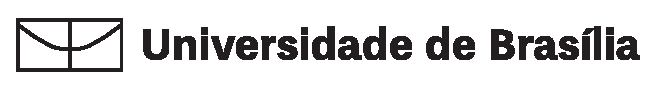
\includegraphics[scale=1]{obj/unb.eps}
\end{flushleft}

	\thispagestyle{empty}

\begin{center}
	
	\vspace{7cm}
	
	{\bf 
		\huge{\sc \edverao\ Escola de Ver\~{a}o em Matem\'{a}tica}\\
		
		\vspace{2cm}
		
		\huge{\sc \edworkshop\ Workshop de Ver\~{a}o em Matem\'{a}tica}}
	
	\vspace{5cm}
	
	\huge{Livro de Resumos}
	
\end{center}

	
\newpage\clearpage
%====================================================================
%							Creditos
%====================================================================


	$\qquad$
	\thispagestyle{empty}
	\begin{flushleft}
		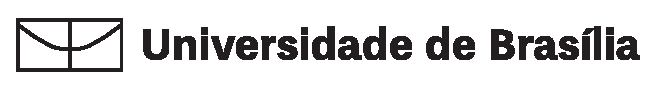
\includegraphics[scale=1]{obj/unb.eps}
		
		\vspace{1.5cm}
		
		\noindent Universidade de Bras\'{i}lia\\
		\noindent Instituto de Ci\^{e}ncias Exatas\\
		\noindent Departamento de Matem\'{a}tica\\
		\noindent Campus Universit\'{a}rio Darcy Ribeiro\\
		\noindent 70910-900 Bras\'{i}lia - DF\\
		
		\vspace{1.15cm}
		
		\noindent \edverao\ Escola de Ver\~{a}o em Matem\'{a}tica\\
		\noindent \edworkshop\ Workshop de Ver\~{a}o em Matem\'{a}tica\\
		
		\vspace{1.15cm}
		
		\noindent Reitor(a) da Universidade de Bras\'{i}lia: \reitor \\
		\noindent Diretor(a) do Instituto de Ci\^{e}ncias Exatas: \dirIE \\
		\noindent Chefe do Departamento de Matem\'{a}tica: \chefMAT \\
		\noindent Coordenador(a) de Extens\~{a}o: \coordext \\
		\noindent Coordenador(a) de P\'{o}s-Gradua\c{c}\~{a}o: \coordpos \\
		
		\vspace{1.15cm}
		
		\noindent Coordenadores da \edverao\ Escola de Ver\~{a}o em Matem\'{a}tica \\e do \edworkshop\ Workshop de Ver\~{a}o em Matem\'{a}tica: \\
		\noindent \coordgeral\\
		\noindent  \coordgerali\\
		\noindent  \coordgeralii
		
		\vspace{1.15cm}
		
		\noindent Coordenadores de \'{A}reas do \edworkshop\ Workshop de Ver\~{a}o em Matem\'{a}tica: \\
		\noindent \'{A}lgebra e Teoria dos N\'{u}meros: \coordalgebra \\
		\noindent An\'{a}lise: \coordanalise \\
		\noindent Educa\c{c}\~{a}o Matem\'{a}tica: \coordedumat\\
		\noindent Geometria: \coordgeometria \\
%		\noindent Matem\'{a}tica Aplicada: \coordmataplic \\
		\noindent Dinâmica de Fluidos: \coorddinflui \\
		\noindent Probabilidade: \coordprobab \\
		\noindent Sistemas Din\^{a}micos:  \coordsistdin \\
		\noindent Teoria da Computa\c{c}\~{a}o: \coordteocomp\\
		\noindent Teoria dos N\'{u}meros: \coordteonumeros\\
	\end{flushleft}
	
	\vspace{1.15cm}
	
	\noindent Elabora\c{c}\~{a}o do Livro de Resumos: \livresumos \\
%	\noindent Apoio \`{a} Elabora\c{c}\~{a}o do Livro de Resumos: \apoio  \\
	\noindent Projeto Gr\'{a}fico da Capa: \artcapa
	
	\vspace{1.15cm}
	
	\begin{center}
		Bras\'{i}lia, mes_realizacao_evento de \ano.
	\end{center}
	
	\newpage\clearpage
	
	
	
	
%====================================================================
%	Prefacio
%====================================================================

	\begin{center}
	%\vspace{1cm}
	\huge{{\bf Pref\'{a}cio}}
	\vspace{1cm}
	\end{center}

Caros participantes,

\vspace{24pt}

\'{E} com enorme prazer que lhes damos as boas-vindas ao \edworkshop\ Workshop de Ver\~{a}o em Matem\'{a}tica, realizado entre os dias \datainic\ e \datafim\ de mes_realizacao_evento de \ano, paralelamente aos cursos da \edverao\ Escola de Ver\~{a}o do Departamento de Matem\'{a}tica da Universidade de Bras\'{i}lia.

\vspace{24pt}

A Escola de Ver\~{a}o do Departamento de Matem\'{a}tica da Universidade de Bras\'{i}lia foi idealizada no in\'{i}cio dos anos 70 e, nestes mais de quarenta anos de tradi\c{c}\~{a}o, tem fomentado em diversos n\'{i}veis o interc\^{a}mbio cient\'{i}fico-cultural entre seus participantes. Estas intera\c{c}\~{o}es acad\^{e}micas s\~{a}o fundamentais para o progresso do conhecimento e para propiciar colabora\c{c}\~{o}es de pesquisa de valor inestim\'{a}vel. De fato, o Programa de P\'{o}s-Gradua\c{c}\~{a}o em Matem\'{a}tica da Universidade de Bras\'{i}lia, atualmente avaliado com nota 7 na CAPES, muito tem se beneficiado de um ambiente acad\^{e}mico ativo e produtivo e, de fato, eventos como o Workshop foram importantes para que nosso programa de p\'{o}s-gradua\c{c}\~{a}o atingisse este n\'{i}vel de excel\^{e}ncia.

\vspace{24pt}

Neste evento ser\~{a}o promovidas palestras de divulga\c{c}\~{a}o cient\'{i}fica e minicursos em diferentes \'{a}reas de interesse, fornecendo aos participantes da Escola de Ver\~{a}o uma vis\~{a}o diversificada sobre variados t\'{o}picos de pesquisa em Matem\'{a}tica, em especial nas \'{a}reas de interesse dos pesquisadores do MAT/UnB. O principal objetivo destas atividades consiste no interc\^{a}mbio e divulga\c{c}\~{a}o de trabalhos desenvolvidos pelos pesquisadores e estudantes de p\'{o}s-gradua\c{c}\~{a}o participantes do evento. Assim, gostar\'{i}amos de agradecer todo o suporte e empenho dos subcoordenadores de \'{a}reas do Workshop e das secretarias de gradua\c{c}\~{a}o e de p\'{o}s-gradua\c{c}\~{a}o do Departamento de Matem\'{a}tica. 

\vspace{24pt}

Agradecemos, em especial, o apoio substancial da Universidade de Bras\'{i}lia, da FAP-DF e da CAPES, que nos concederam recursos essenciais para a organiza\c{c}\~{a}o deste evento.

\vspace{24pt}

Finalmente, apenas nos resta desej\'{a}-los uma excelente estadia em Bras\'{i}lia e na Universidade de Bras\'{i}lia. Assistam a muitas palestras, interajam com v\'{a}rias pessoas, aprendam muita matem\'{a}tica e, acima de tudo, \textit{\sc divirtam-se}!

\vspace{24pt}

Um grande abra\c{c}o,

\vspace{24pt}

\begin{center}
	\coordgeral, \coordgerali\ e \coordgeralii\\ 
	Coordenadores do \edworkshop\ Workshop de Ver\~{a}o em Matem\'{a}tica\\
	e da \edverao\ Escola de Ver\~{a}o do MAT-UnB
\end{center}

%\vfill

%====================================================================
%	Fim Creditos & Prefacio
%====================================================================

\restoregeometry